% !TEX program = XeLaTeX
% !TEX encoding = UTF-8
\documentclass[UTF8,nofonts]{article}
%{ctexart}


%\setCJKmainfont[BoldFont=FandolSong-Bold.otf,ItalicFont=FandolKai-Regular.otf]{FandolSong-Regular.otf}
%\setCJKsansfont[BoldFont=FandolHei-Bold.otf]{FandolHei-Regular.otf}
%\setCJKmonofont{FandolFang-Regular.otf}

\usepackage{url}
\usepackage{cancel}
\usepackage{xspace}
\usepackage{graphicx}
\usepackage{multicol}
\usepackage{multirow}
\usepackage{subfig}
\usepackage{amsmath}
\usepackage{amssymb}
\usepackage[a4paper, width=186mm, top=18mm, bottom=18mm, includeheadfoot]{geometry}
%\usepackage[a4paper, width=140mm, top=18mm, bottom=22mm, includeheadfoot]{geometry}
\usepackage{booktabs}
\usepackage{array}
\usepackage{verbatim}
\usepackage{caption}
\usepackage{natbib}
\usepackage{booktabs}
\usepackage{float}
\usepackage{pdflscape}
\usepackage{mathtools}
\usepackage[usenames, dvipsnames]{xcolor}
\usepackage{afterpage}
\usepackage{pgf}
\usepackage{tikz}
\usepackage{dirtree}
\usepackage[style=american]{csquotes}
\usepackage{amsfonts}
\usepackage{tikz}
\usepackage{tkz-graph}
\usetikzlibrary{arrows,decorations.pathmorphing,automata,positioning,backgrounds,fit,shapes.symbols,chains,intersections}

\newtheorem{definition}{Definition}[section]
\newtheorem{theorem}{Theorem}[section]
\newtheorem{lemma}{Lemma}
\newtheorem{proof}{Proof} [section]



\usepackage[toc, page, title, titletoc, header]{appendix}
\usepackage{marginnote}
\usepackage{tablefootnote}

%\renewcommand\appendixname{附\ 录}
%\renewcommand\appendixpagename{附\ 录}
%\renewcommand\appendixtocname{附\ 录}
\renewcommand\abstractname{Abstract}


\usepackage{perpage} %the perpage package
\MakePerPage{footnote} %the perpage package command

\usetikzlibrary{shapes.geometric}%
\usepackage{color}
%\usepackage[pages=some, placement=top]{background}
\usepackage{eso-pic}
\usepackage[final]{pdfpages}

%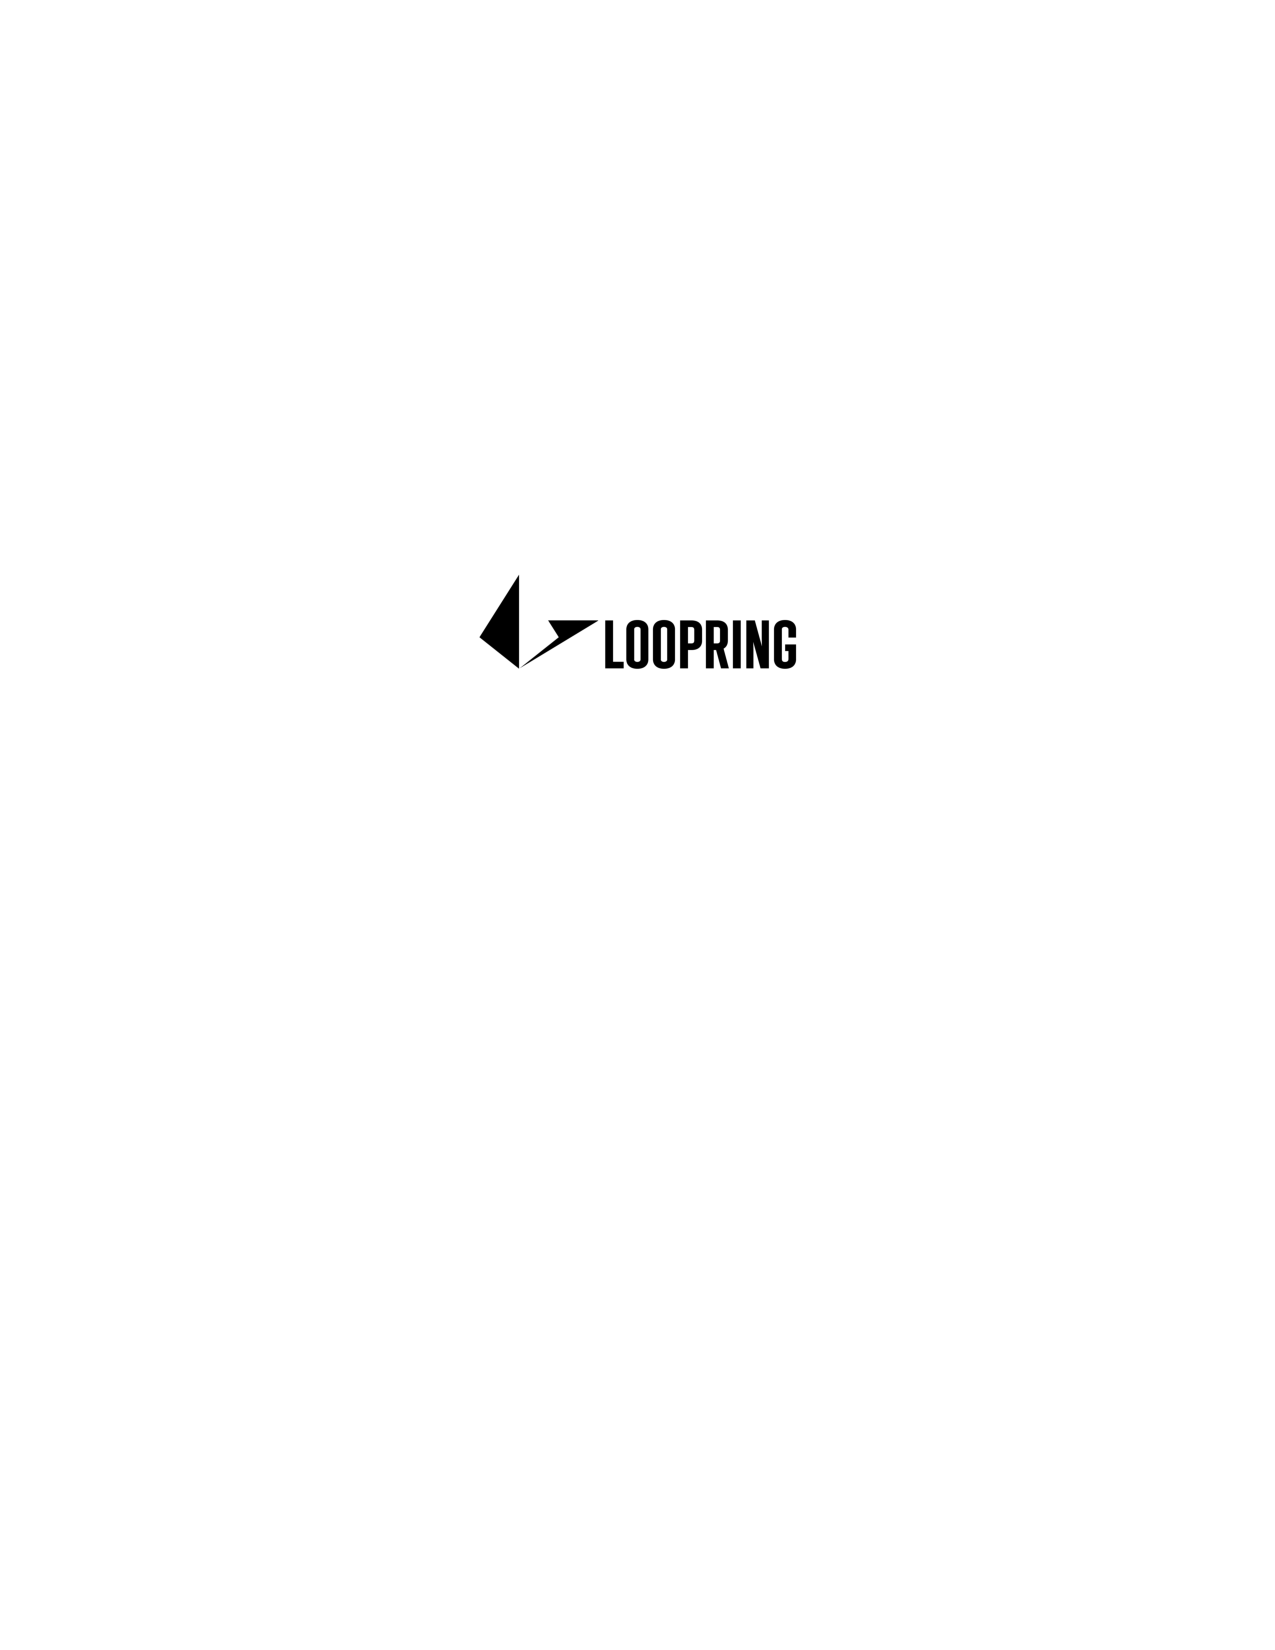
\includepdf[pages=1]{cover}
\hyphenpenalty=750

\title{\textbf{Loopring:}\\\textbf{A Decentralized Token Exchange Protocol}}
\author{
  Daniel Wang\\
  \texttt{daniel@loopring.org}\\
  \and
  	Jay Zhou\\
  	\texttt{jay@loopring.org}\\
  	\and
  	Alex Wang\\
  	\texttt{alex@loopring.org}\\
  	\and
  	Matthew Finestone\\
  	\texttt{matt.finestone@gmail.com}\\ 
  \\
  \texttt{https://loopring.org}
 }

\makeatletter
\def\CTEX@section@format{\Large\bfseries}
\makeatother

\makeatletter
\newenvironment{tablehere}
 {\def\@captype{table}}
 {}

\newenvironment{figurehere}
 {\def\@captype{figure}}
 {}
\makeatother
%
%\newcommand\BackgroundPic{%
%\put(0, 0){%
%\parbox[b][\paperheight]{\paperwidth}{%
%\vfill
%\centering
%\includegraphics[width=\paperwidth, height=\paperheight, %
%%keepaspectratio]{images/background.jpg}%
%]{images/background.jpg}%
%\vfill
%}}}


\begin{document}
%\AddToShipoutPicture{\BackgroundPic}
\maketitle


\begin{abstract}
Loopring is an open protocol for building decentralized exchanges. Loopring operates as a public set of smart contracts responsible for trade and settlement, with an off-chain group of actors aggregating and communicating orders. The protocol is free, extensible, and serves as a standardized building block for decentralized applications (dApps) that incorporate exchange functionality. Its interoperable standards facilitate trustless, anonymous trading. An important improvement over current decentralized exchange protocols is the ability for orders to be mix-and-matched with other, dissimilar orders, obviating the constraints of two-token trading pairs and drastically improving liquidity. Loopring also employs a unique and robust solution to prevent front-running: the unfair attempt to submit transactions into a block quicker than the original solution provider. Loopring is blockchain agnostic, and deployable on any blockchain with smart contract functionality. At the time of writing, it's operable on Ethereum \cite{buterin2017ethereum} \cite{wood2014ethereum} and Qtum \cite{dai2017smart} with NEO \cite{atterlonn2018distributed} under construction.
\end{abstract}



\begin{multicols}{2}
\section{Introduction\label{sec:introduction}}

With the proliferation of blockchain-based assets, the need to exchange these assets amongst counterparties has significantly increased. As thousands of new tokens are introduced - including the tokenization of traditional assets - this need is magnified. Whether exchanging tokens for speculative trading motivations, or converting to access networks via their native utility tokens, the ability to exchange one cryptoasset for another is foundational for the larger ecosystem. Indeed, there is a potential energy in assets \cite{desotocapital}, and realizing this energy - unlocking capital - requires not only asserting ownership, which blockchains have immutably allowed for, but the ability to freely transfer and transform these assets.
 
As such, the trustless exchange of tokens (value) is a compelling use case for blockchain technology. Until now, however, crypto enthusiasts have largely settled for trading tokens on traditional centralized exchanges. The Loopring protocol is needed because, just as Bitcoin \cite{nakamoto2008bitcoin} dutifully emphasized that, in regards to peer-to-peer electronic cash, \enquote{the main benefits are lost if a trusted third party is still required to prevent double-spending}, so too are the main benefits of decentralized assets lost if they must pass through trusted, gated, centralized exchanges.

Trading decentralized tokens on centralized exchanges doesn't make sense from a philosophical perspective, as it fails to uphold the virtues these decentralized projects espouse. There are also numerous practical risks and limitations in using centralized exchanges which are described below. Decentralized exchanges (DEXs) \cite{schuh2015bitshares} \cite{bancor} \cite{kyber} have sought to address these issues, and in many cases have succeeded in alleviating security risks by using blockchains for disintermediation. However, as DEX capability becomes crucial infrastructure for the new economy, there is substantial room for performance improvement. Loopring aims to provide modular tools for said infrastructure with its dApp agnostic open protocol.

\section{Current Exchange Landscape\label{sec:current_exchange_landscape}}

\subsection{Inadequacies of Centralized Exchanges}
The three primary risks of centralized exchanges are; 1) Lack of security, 2) Lack of transparency, and 3) Lack of liquidity.

\textbf{Lack of Security} arises from users typically surrendering control of their private-keys (funds) to one centralized entity. This exposes users to the possibility that centralized exchanges fall prey to malicious hackers. The security and hacking risks facing all centralized exchanges are well known \cite{coincheckhack}  \cite{mcmillan2014inside}, yet are often accepted as \enquote{table stakes} for token trading. Centralized exchanges continue to be honeypots for hackers to attack as their servers have custody over millions of dollars of user funds. Exchange developers can also make honest, accidental errors with user funds. Simply, users are not in control of their own tokens when deposited at a centralized exchange.

\textbf{Lack of Transparency} exposes users to the risk of dishonest exchanges acting unfairly. The distinction here is by the exchange operator's malicious intentions, as users are not truly trading their own assets on centralized exchanges, but rather, an IOU. When tokens are sent to the exchange's wallet, the exchange takes custody, and offers an IOU in its place. All trades are then effectively between users' IOUs. To withdraw, users redeem their IOU with the exchange, and receive their tokens to their external wallet address. Throughout this process there is a lack of transparency, and the exchange can shutdown, freeze your account, go bankrupt, etc. It is also possible that they use user assets for other purposes while in custody, such as lending them out to third parties. Lack of transparency can cost users without a total loss of funds, such as in higher trading fees, delays at peak demand, regulatory risk, and orders being front ran.

\textbf{Lack of Liquidity.} From the point of view of exchange operators, fragmented liquidity inhibits entry by new exchanges because of two winner-takes-all scenarios. First, the exchange with the greatest number of trading pairs wins, because users find it desirable to conduct all their trades on one exchange. Second, the exchange with the largest order book wins, because of favorable bid-ask spreads for each trading pair. This discourages competition from newcomers because it is difficult for them to build up initial liquidity. As a result, many exchanges command a high market share despite user complaints and even major hacking incidents. It's worth noting that as centralized exchanges win market share, they become an ever-larger hacking target.

From the point of view of users, fragmented liquidity significantly reduces user experience. In a centralized exchange, users are only able to trade within the exchange's own liquidity pools, against its own order book, and between its supported token pairs. To trade token \verb|A| for token \verb|B|, users must go to an exchange that supports both tokens or register at different exchanges, disclosing personal information. Users often need to execute preliminary or intermediate trades, typically against BTC or ETH, paying bid-ask spreads in the process. Finally, the order books may not be deep enough to complete the trade without material slippage. Even if the exchange purports to process large volumes, there is no guarantee that this volume and liquidity is not fake \cite{fakevolume}.

The result is disconnected silos of liquidity and a fragmented ecosystem that resembles the legacy financial system, with significant trading volume centralized on few exchanges. The global liquidity promises of blockchains hold no merit within centralized exchanges.

\subsection{Inadequacies of Decentralized Exchanges}
Decentralized exchanges differ from centralized exchanges in part because users maintain control of their private-keys (assets) by performing trades directly on the underlying blockchain. By leveraging the trustless technology of cryptocurrencies themselves, they successfully mitigate many of the abovementioned risks surrounding security. However, problems persist in regards to performance and structural limitations. 

Liquidity often remains an issue as users must search for counterparties across disparate liquidity pools and standards. Fragmented liquidity effects are present if DEXs or dApps at large don't employ consistent standards to interoperate, and if orders are not shared/propagated across a wide network. The liquidity of limit order books, and, specifically, their resiliency -- how fast filled limit orders are regenerated -- can significantly affect optimal trading strategies \cite{limitorderliquidity}. The absence of such standards has resulted not only in reduced liquidity, but also exposure to an array of potentially insecure proprietary smart contracts.

Furthermore, since trades are performed on chain, DEXs inherit the limitations of the underlying blockchain, namely: scalability, delays in execution (mining), and costly modifications to orders. Thus, blockchain order books do not scale particularly well, as executing code on the blockchain incurs a cost (gas), making multiple order-cancellation cadences prohibitively expensive. 

Finally, because blockchain order books are public, the transaction to place an order is visible by miners as it awaits being mined into the next block and placed into an order book. This delay exposes the user to the risk of being front run and having the price or execution move against him.

\subsection{Hybrid Solutions}
For the above reasons, purely blockchain-based exchanges have limitations that make them uncompetitive with centralized exchanges. There is a tradeoff between on-chain inherent trustlessness, and centralized exchange speed and order flexibility. Protocols such as Loopring and 0x \cite{warren20170x} extend a solution of on-chain settlement with off-chain order management. These solutions revolve around open smart contracts, but navigate scalability limitations by performing several functions off-chain and giving nodes flexibility in fulfilling critical roles for the network. However, drawbacks remain for the hybrid model as well \cite{costofdecent}. The Loopring protocol proposes meaningful differences in our approach to a hybrid solution throughout this paper.


\section{Loopring Protocol\label{sec:loopring_protocol}}
Loopring is not a DEX, but a modular protocol for building DEXs on multiple blockchains. We disassemble the component parts of a traditional exchange and offer a set of public smart contracts and decentralized actors in its place. The roles in the network include wallets, relays, liquidity-sharing consortium blockchains, order book browsers, Ring-Miners, and asset tokenization services. Before defining each, we should first understand Loopring orders. 

\subsection{Order Ring\label{sec:order_ring}}
Loopring orders are expressed in what we call a Unidirectional Order Model (UDOM)\cite{coinport2014udom}. UDOM expresses orders as token exchange requests, \verb|amountS|/\verb|amountB|, (amount to sell/buy)  instead of bids and asks. Since every order is just an exchange rate between two tokens, a powerful feature of the protocol is the mixing and matching of multiple orders in circular trade. By using up to 16 orders instead of a single trading pair, there is a dramatic increase in liquidity and potential for price improvement. 

\begin{center}
\begin{figurehere}
\centering
\tikzstyle{block} = [draw, fill=blue!20, rectangle, 
    minimum height=3em, minimum width=6em]
\tikzstyle{sum} = [draw, fill=blue!20, circle, node distance=1cm]
\tikzstyle{input} = [coordinate]
\tikzstyle{output} = [coordinate]
\tikzstyle{pinstyle} = [pin edge={to-,thin,black}]

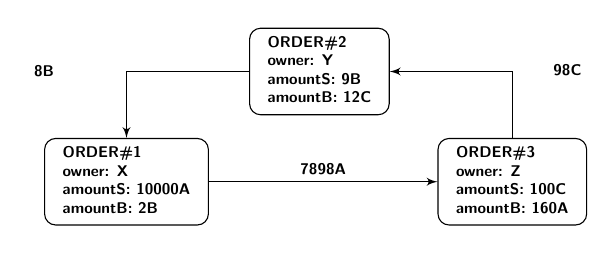
\begin{tikzpicture}[
    auto, 
    node distance=2cm,
    >=latex',
    font=\bfseries\footnotesize\sffamily,
    order/.style={
		scale=0.7,
		rectangle,
		rounded corners,
		draw=black, 
		text centered,
%		text width=5cm,
		minimum height=12mm,
		fill=white
	},
	label/.style={
		scale=0.7
	}
  ]
    % We start by placing the blocks

  \node [order] (order2) 
 {%
 \begin{tabular}{l}
  \textbf{ORDER\#2}\\
  \textbf{owner: Y}\\
  \textbf{amountS: 9B}\\
  \textbf{amountB: 12C}
 \end{tabular}
 };
 
  \node [order, below of=order2, xshift=-3.5cm] (order1) 
 {%
 \begin{tabular}{l}
  \textbf{ORDER\#1}\\
  \textbf{owner: X}\\
  \textbf{amountS: 10000A}\\
  \textbf{amountB: 2B}
 \end{tabular}
 };
 
 
  \node [order, below of=order2, xshift=3.5cm] (order3) 
 {%
 \begin{tabular}{l}
  \textbf{ORDER\#3}\\
  \textbf{owner: Z}\\
  \textbf{amountS: 100C}\\
  \textbf{amountB: 160A}
 \end{tabular}
 };
 
 \draw [draw,->] (order1) -- node [label] {\textbf{7898A}} (order3);
 \draw [draw,->] (order2) -| node [label, xshift=-1.8cm] {\textbf{8B}} (order1);
 \draw [draw,->] (order3) |- node [label, xshift=1cm, yshift=0.24cm] {\textbf{98C}} (order2);

\end{tikzpicture}

\caption{An order-ring of 3 orders}
\label{fig:ring}
\end{figurehere}
\end{center}


The above figure shows an order-ring of 3 orders. Each order's token to sell (\verb|tokenS|) is another order's token to buy (\verb|tokenB|). It creates a loop that allows each order to exchange their desired tokens without requiring an opposing order for its pair. Traditional order pair trades can, of course, still be executed, in what is essentially a special case of an order-ring. 

\begin{definition}[order-ring] Let $C_{0}$, $C_{1}$, $\cdots$, $C_{n-1}$ be $n$ different tokens, $O_{0\rightarrow 1}$, $\cdots$, $O_{i\rightarrow i\oplus 1}$, $\cdots$, $O_{n-1 \rightarrow 0}$ be $n$ orders. Those orders can form a order-ring for trading:
$$O_{0\rightarrow 1} \rightarrow \cdots \rightarrow O_{i\rightarrow i\oplus 1} \rightarrow \cdots \rightarrow O_{n-1\rightarrow 0} \text{, }$$
where $n$ is the length of the order-ring, and $i\oplus 1 \equiv i+1 \mod n$.
\end{definition}

An order-ring is valid when all component transactions can be executed at an exchange rate equal to or better than the original rate specified implicitly by the user. To verify order-ring validity, Loopring protocol smart contracts must receive order-rings from ring-miners where the product of the original exchange rates of all orders is equal to or greater than 1.

Let's assume Alice and Bob want to trade their token \verb|A| and \verb|B|. Alice has 15 token \verb|A| and she wants 4 token \verb|B| for them; Bob has 10 token \verb|B|  and he wants 30 token \verb|A| for them.

Who is buying and who is selling? This depends only on the asset we fix to give price quotations. If token \verb|A| is the reference, then Alice is buying token \verb|B| for the price of ${15 \over 4} = 3.75$\verb|A|, while Bob is selling 10 token \verb|B| for the price of ${30 \over 10} = 3.00$\verb|A|. In the case of fixing token \verb|B| as reference, we say that Alice is selling 15 token \verb|A| for the price of ${4\over 15}=0.26666667$\verb|B| and Bob is buying 10 token \verb|A| for the price of ${10 \over 30}=0.33333334$\verb|B|. Hence, who's the buyer or seller is arbitrary.

In the first situation Alice is willing to pay a higher price ($3.75$\verb|A|) than the price Bob is selling his tokens for ($3.00$\verb|A|), while in the second situation Bob is willing to pay a higher price ($0.33333334$\verb|B|) than the price Alice is selling her tokens for ($0.26666667$\verb|B|). It is clear that a trade is possible whenever the buyer is willing to pay an equal or higher price than the seller's price.

\begin{equation}
{{15\over 4} \over {30\over 10}} = {{10\over 30} \over {4\over 15}}={15 \over 4} \cdot {10 \over 30} = 1.25 > 1
\end{equation}

Thus, for a set of $n$ orders to be able to be filled, fully or partially, we need to know if the product of each one of the exchange rates as buy orders results in a number greater or equal to 1. If so, all the $n$ orders can be either partially, or totally filled \cite{supersymmetry}.

If we introduce a third counterparty, Charlie, such that  Alice wants to give $x_1$ token \verb|A| and receive $y_1$ token \verb|B|, Bob wants to give $x_2$ token \verb|B| and receive $y_2$ token \verb|C|, and Charlie wants to give $x_3$ token \verb|C| and receive $y_3$ token \verb|A|. The necessary tokens are present, and the trade is possible if:

\begin{equation}
{{x_1 \cdot x_2 \cdot x_3 \over y_1 \cdot y_2 \cdot y_3} \geq 1}
\end{equation}


See section \ref{anatomy} for more details about Loopring's orders.



\section{Ecosystem Participants\label{sec:ecosystem}}
The following ecosystem participants jointly provide all functionalities a centralized exchange has to offer. 

\begin{itemize}

\item \textbf{Wallets}: A common wallet service or interface that gives users access to their tokens and a way to send orders to the Loopring network. Wallets will be incentivized to produce orders by sharing fees with ring-miners (see section \ref{sec:token}). With the belief that the future of trading will take place within the safety of individual user's wallets, connecting these liquidity pools through our protocol is paramount.

\item \textbf{Consortium Liquidity Sharing Blockchain/Relay-Mesh}: A relay-mesh network for order \& liquidity sharing. When nodes run Loopring relay software, they are able to join an existing network and share liquidity with other relays over a consortium blockchain. The consortium blockchain we are building as a first implementation has near real time order sharing (1-2 second blocks), and trims old history to allow for faster download by new nodes. Notably, relays need not join this consortium; they can act alone and not share liquidity with others, or, they can start and manage their own liquidity sharing network.

\item \textbf{Relays/Ring-Miners}: Relays are nodes that receive orders from wallets or the relay-mesh, maintain public order books and trade history, and optionally broadcast orders to other relays (via any arbitrary off-chain medium) and/or relay-mesh nodes. Ring-mining is a feature -- not a requirement -- of relays. It is computationally heavy and is done completely off-chain. We call relays with the ring-mining feature turned on \enquote{Ring-Miners}, who produce order-rings by stitching together disparate orders. Relays are free in (1) how they choose to communicate with one another, (2) how they build their order books, and (3) how they mine order-rings (mining algorithms).

\item \textbf{Loopring Protocol Smart Contracts (LPSC)}: A set of public and free smart contracts that checks order-rings received from ring-miners, trustlessly settles and transfers tokens on behalf of users, incentivizes ring-miners and wallets with fees, and emits events. Relays/order browsers listen to these events to keep their order books and trade history up to date. See appendix \ref{app:protocol_ethereum} for details.

\item \textbf{Asset Tokenization Services (ATS)}: A bridge between assets that cannot be directly traded on Loopring. They are centralized services run by trustworthy companies or organizations. Users deposit assets (real, fiat or tokens from other chains) and get tokens issued, which can be redeemed for the deposit in the future. Loopring is not a cross-chain exchange protocol (until a suitable solution exists), but ATS enable trading of ERC20 tokens \cite{ERC20} with physical assets as well as assets on other blockchains. 

\end{itemize}


\section{Exchange Process\label{sec:process}}



\begin{enumerate} 


\item \textbf{Protocol Authorization}: In figure \ref{fig:process}, user \verb|Y| who wants to exchange tokens authorizes the LPSC to handle \verb|amountS| of token \verb|B| the user wants to sell. This does not lock the user's tokens, who remains free to move them while the order is processed.

\item \textbf{Order Creation}: The current rate and order book for token \verb|B| vs token \verb|C|, are provided by relays or other agents hooked up to the network, such as order book browsers. User \verb|Y| places an order (limit order) specifying \verb|amountS| and \verb|amountB| and other parameters through any integrated wallet interface. An amount of LRx can be added to the order as a fee for ring-miners; higher LRx fee means a better chance to be processed earlier by ring-miners. The order's hash is signed with user \verb|Y|'s private-key.

\item \textbf{Order Broadcast}: The wallet sends the order and its signature to one or more relays. Relays update their public order book. The protocol doesn't require order books to be built in a certain way, such as first-come-first-serve. Instead, relays have the power to make their own design decisions in building their order books.

\item \textbf{Liquidity Sharing}: Relays broadcast the order to other relays through any arbitrary communication medium. Once again, there is flexibility how/whether nodes interact. To facilitate a certain level of network connectivity, there is a built-in liquidity sharing relay-mesh using a consortium blockchain. As mentioned in the prior section, this relay-mesh is optimized for speed and inclusivity.

\begin{center}
\begin{figurehere}
\centering
\tikzstyle{block} = [draw, fill=blue!20, rectangle, 
    minimum height=3em, minimum width=6em]
\tikzstyle{sum} = [draw, fill=blue!20, circle, node distance=1cm]
\tikzstyle{input} = [coordinate]
\tikzstyle{output} = [coordinate]
\tikzstyle{pinstyle} = [pin edge={to-,thin,black}]

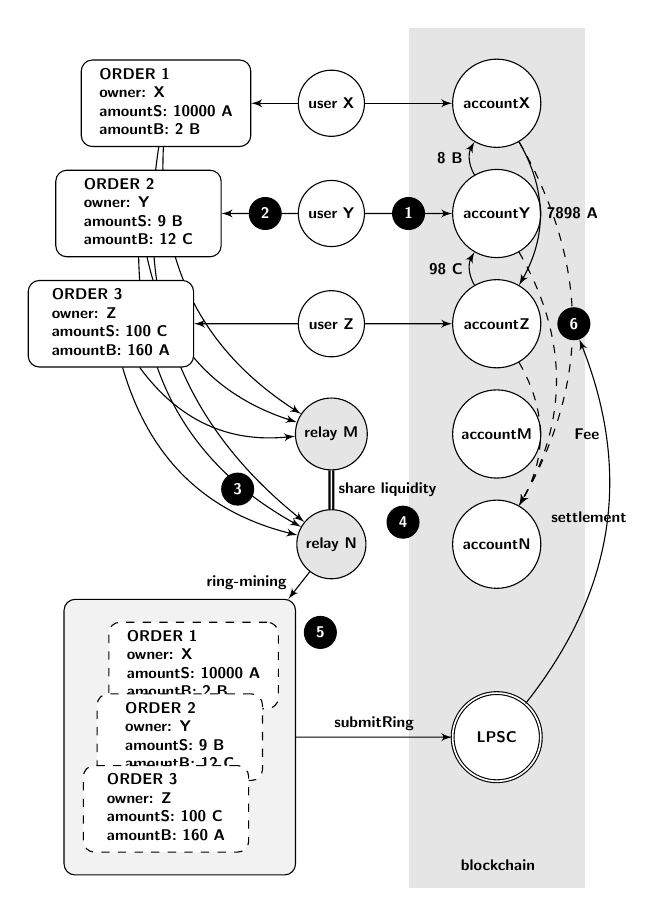
\begin{tikzpicture}[
    auto, 
    scale=0.7,
    node distance=2cm,
    >=latex',
    font=\bfseries\footnotesize\sffamily,
    order/.style={
		rectangle,
		scale=0.7,
		rounded corners,
		draw=black, 
		text centered,
%		text width=5cm,
		minimum height=12mm,
		minimum width=30mm,
		fill=white
	},
	role/.style={
		circle,
		scale=0.7,
		draw=black, 
		text centered,
%		text width=5cm,
		minimum height=12mm,
		minimum width=12mm,
		fill=white
	},
	steps/.style={
		circle,
		scale=0.7,
		draw=black, 
		text centered,
%		text width=5cm,
%		minimum height=12mm,
%		minimum width=12mm,
		fill=black,
		text=white
	},
	account/.style={
		circle,
		scale=0.7,
		draw=black, 
		text centered,
%		text width=5cm,
		minimum height=16mm,
		minimum width=16mm,
		fill=white
	},
	label/.style={
	  scale=0.7
    }
  ]

 
 \node [role] (user1)  {user X};
 \node [role, below of=user1] (user2)  {user Y};
 \node [role, below of=user2] (user3)  {user Z};
 \node [role, below of=user3, fill=gray!20] (relay1)  {relay M};
 \node [role, below of=relay1, fill=gray!20] (relay2)  {relay N};

 
 \node [order, left of=user1, xshift=-1cm] (order1) 
 {%
 \begin{tabular}{l}
  \textbf{ORDER 1}\\
  \textbf{owner: X}\\
  \textbf{amountS: 10000 A}\\
  \textbf{amountB: 2 B}
 \end{tabular}
 };
 
 \draw [draw, ->]  (user1) -- (order1) [label]{};
 \draw [bend right,->] (order1) to node [auto, scale=0.7] {} (relay1);
 \draw [bend right,->] (order1) to node [auto, scale=0.7] {} (relay2);
% \draw [draw, ->]  (order1) |- (relay1) [label]{};
% \draw [draw, ->]  (order1) |- (relay2) [label]{};
 
 \node [order,left of=user2, xshift=-1.5cm] (order2) 
 {%
 \begin{tabular}{l}
  \textbf{ORDER 2}\\
  \textbf{owner: Y}\\
  \textbf{amountS: 9  B}\\
  \textbf{amountB: 12 C}
 \end{tabular}
 };
 \draw [draw, ->]  (user2) -- (order2) [label]{};
 \draw [bend right,->] (order2) to node [auto, scale=0.7] {} (relay1);
 \draw [bend right,->] (order2) to node [auto, scale=0.7] {} (relay2);
% \draw [draw, ->]  (order2) |- (relay1) [label]{};
% \draw [draw, ->]  (order2) |- (relay2) [label]{};
% 
\node [order, left of=user3, xshift=-2cm] (order3) 
 {%
 \begin{tabular}{l}
  \textbf{ORDER 3}\\
  \textbf{owner: Z}\\
  \textbf{amountS: 100 C}\\
  \textbf{amountB: 160 A}
 \end{tabular}
 };
 \draw [draw, ->]  (user3) -- (order3) [label]{};
 \draw [bend right,->] (order3) to node [auto, scale=0.7] {} (relay1);
 \draw [bend right,->] (order3) to node [auto, scale=0.7] {} (relay2);
% \draw [draw, ->]  (order3) |- (relay1) [label]{};
% \draw [draw, ->]  (order3) |- (relay2) [label]{};
 
% // The Ring
\node [order, 
yshift=-1.5cm,
xshift=-2.75cm,
below of=relay2,
fill=gray!10,
minimum width=4.2cm,
minimum height=5cm] (ring) {};


\node [order, dashed, below of=relay2,yshift=-0.2cm,xshift=-2.5cm] (order11) 
 {%
 \begin{tabular}{l}
  \textbf{ORDER 1}\\
  \textbf{owner: X}\\
  \textbf{amountS: 10000 A}\\
  \textbf{amountB: 2 B}
 \end{tabular}
 };
 \node [order, dashed,below of=order11,xshift=-0.25cm,yshift=0.7cm] (order21) 
 {%
 \begin{tabular}{l}
  \textbf{ORDER 2}\\
  \textbf{owner: Y}\\
  \textbf{amountS: 9  B}\\
  \textbf{amountB: 12 C}
 \end{tabular}
 };
\node [order, dashed,below of=order21,xshift=-0.25cm,yshift=0.7cm] (order31) 
 {%
 \begin{tabular}{l}
  \textbf{ORDER 3}\\
  \textbf{owner: Z}\\
  \textbf{amountS: 100 C}\\
  \textbf{amountB: 160 A}
 \end{tabular}
 };
 
 % // The blockchain
\node [
rectangle,
fill=gray!20, 
right of=user1,
yshift=-4.5cm,
xshift=0.1cm,
scale=0.7,
minimum width=3.2cm,
minimum height=15.6cm] (blockchain) {\parbox[b][15cm]{1.3cm}{blockchain}};
% blockchain accounts
  \node [account, right of=user1, xshift=1cm] (account1)  {accountX};
  \node [account, right of=user2, xshift=1cm] (account2)  {accountY};
  \node [account, right of=user3, xshift=1cm] (account3)  {accountZ};
  \node [account, right of=relay1, xshift=1cm] (account4)  {accountM};
  \node [account, right of=relay2, xshift=1cm] (account5)  {accountN};
  \node [account, double, below of=account5, yshift=-1.5cm] (psc)  {LPSC};
  
 \draw [draw, ->]  (user1) -- (account1) [label]{};
 \draw [draw, ->]  (user2) -- (account2) [label]{};
 \draw [draw, ->]  (user3) -- (account3) [label]{};
% \draw [draw, ->]  (relay1) -- (account4) [label]{};
% \draw [draw, ->]  (relay2) -- (account5) [label]{};
 \draw [draw, double, thick]  (relay1) to node [auto, scale=0.7] {share liquidity}  (relay2) [label]{};
% \draw [draw, ->]  (relay1) -- (ring) [label]{};
 \draw [draw, ->]  (relay2) to node [auto, scale=0.7, xshift=-1.8cm, yshift=0.3cm] {ring-mining}  (ring) [label]{};
 \draw [draw, ->]  (ring) to node [auto, scale=0.7] {submitRing} (psc) [label]{};
 
 \draw [bend left,->] (account1) to node [auto, scale=0.7] {\textbf{7898 A}} (account3);
 \draw [bend left,->] (account2) to node [auto, scale=0.7] {\textbf{8 B}} (account1);
 \draw [bend left,->] (account3) to node [auto, scale=0.7] {\textbf{98 C}} (account2);
 
 \draw [bend left,->, dashed] (account1) to node [auto, scale=0.7] {} (account5);
 \draw [bend left,->, dashed] (account2) to node [auto, scale=0.7] {} (account5);
 \draw [bend left,->, dashed] (account3) to node [auto, scale=0.7, xshift=.5cm] {\textbf{Fee}} (account5);
  
  
% \draw [draw,->] (order1) -- node [label] {\textbf{7898 A}} (order3);
% \draw [draw,->] (order2) -| node [label, xshift=-1.8cm] {\textbf{8 B}} (order1);
% \draw [draw,->] (order3) |- node [label, xshift=1cm, yshift=0.24cm] {\textbf{98 C}} (order2);

\node [steps, right of=user2, xshift=-0.6cm] () {1};
\node [steps, left of=user2, xshift=0.8cm] () {2};
\node [steps, left of=relay2, xshift=0.3cm, yshift=1cm] () {3};
\node [steps, left of=relay1, xshift=3.3cm, yshift=-1.6cm] () {4};
\node [steps, below of=relay2, xshift=-0.2cm, yshift=0.4cm] () {5};
\node [steps, right of=account3, xshift=-0.6cm] (step5) {6};

 \draw [bend right, ->]  (psc) to node [auto, scale=0.7, xshift=0.5cm] {settlement} (step5) [label]{};
 
\end{tikzpicture}

\caption{Loopring Exchange Process}
\label{fig:process}
\end{figurehere}
\end{center}



\item \textbf{Ring-Mining (Order Matching)}:  Ring-miners try to fill the order fully or partially at the given exchange rate or better by matching it with multiple other orders. Ring-mining is the main reason why the protocol is able to provide high liquidity over any pair. If the executed rate is better than what user Y specified, margin is shared amongst all orders in the order-ring. As a reward, the ring-miner chooses between claiming part of the margin (Margin-Split, and giving back the LRx to the user), or simply keeping the LRx fee.

\item \textbf{Verification \& Settlement}: The order-ring is received by LPSC. It makes multiple checks to verify the ring-miner supplied data and determines if the order-ring can be settled fully or partially (depending on the fill rate of orders in-ring and tokens in users' wallets). If all checks are successful, the contract atomically transfers the tokens to users and pays the ring-miner and wallet fees at the same time. If user \verb|Y|'s balance as determined by the LPSC is insufficient, it will be considered scaled-down: a scaled-down order will automatically scale up to its original size if sufficient funds are deposited to its address, unlike a cancellation, which is a one way manual operation and cannot be reversed.


\end{enumerate}





%
%\end{multicols}
%
%\begin{center}
%\begin{figurehere}
%\includegraphics[height=8cm]{images/en_protocol.png}
%\caption{Loopring Trading Process}
%\label{fig: Loopringrotocol}
%\end{figurehere}
%\end{center}
%
%\begin{multicols}{2}

\section{Operational Flexibility\label{sec:business_model}}
It's important to note that Loopring's open standard allows participants significant flexibility in how they operate. Actors are free to implement novel business models and provide value for users, earning LRx fees on volume or other metrics in the process (if they so choose). The ecosystem is modular and meant to support participation from a multitude of applications.


\subsection{Order Book\label{sec:order_book}}
Relays can design their order books in any number of ways to display and match users' orders. A first implementation of our own order book follows an OTC model, where limit orders are positioned based on price alone. Timestamps of orders, in other words, have no bearing on the order book. However, a relay is free to design their order book in such a way as to emulate a typical centralized exchange's matching engine, where orders are ranked by price, while respecting timestamps as well. If a relay was inclined to offer this type of order book, they can own/integrate with a wallet, and have those wallet orders sent solely to the single relay, who would then be able to match orders based on time. Any such configuration is possible.


Whereas other DEX protocols at times require Relays to have resources - initial token balances to place taker orders - Loopring Relays need only find matchable orders to consummate a trade, and can do so without initial tokens.

\subsection{Liquidity Sharing\label{sec:liquidity_sharing}}
Relays are free to design how they share liquidity (orders) with each other. Our consortium blockchain is but one solution to accomplish this, and the ecosystem is free to network and communicate as they wish. Besides joining a consortium blockchain, they can build and manage their own, creating rules/incentives as they see fit. Relays can also work alone, as seen in the time-sensitive wallet implementation. Of course, there are clear advantages in communicating with other Relays in pursuit of network effects, however, different business models could merit peculiar sharing designs and split fees in any number of ways.


\section{Protocol Specification\label{sec:protocol}}

\subsection{Anatomy of an Order\label{anatomy}}
An order is a pack of data that describes the intent of the user's trade. A Loopring order is defined using the Uni-Directional Order Model, or UDOM, as follows:

\begin{verbatim}
  message Order {
    address protocol;
    address owner;
    address tokenS;
    address tokenB;
    uint256 amountS;
    uint256 amountB;
    unit256 lrcFee
    unit256 validSince; // Seconds since epoch
    unit256 validUntil; // Seconds since epoch
    uint8   marginSplitPercentage;  // [1-100]
    bool    buyNoMoreThanAmountB;
    uint256 walletId;
    // Dual-Authoring address
    address authAddr;
   	// v, r, s are parts of the signature
    uint8   v;       
    bytes32 r;
    bytes32 s;
    // Dual-Authoring private-key,
    // not used for calculating order's hash,
    // thus it is NOT signed.
    string  authKey;          
  }
\end{verbatim}


To ensure the origin of the order, it is signed against the hash of its parameters, excluding \verb|authAddr|, with the user's private-key. The \verb|authAddr| parameter is used for signing  order-rings that this order is part of, which prevents front-running. Please reference section \ref{sec:dual_authoring} for more details. The signature is represented by the \verb|v|, \verb|r|, and \verb|s| fields, and is sent alongside the order parameters over the network. This guarantees the order stays immutable during its whole lifetime. Even though the order never changes, the protocol can still compute its current state based on the balance of its address along with other variables.



UDOM doesn't include a price (which must be a floating-point number by nature), but, instead uses the term \verb|rate| or $r$, which is expressed as \verb|amountS|/\verb|amountB|. The rate is not a floating-point number but an expression that will only be evaluated with other unsigned integers on demand, to keep all intermediate results as unsigned integers and increase calculation accuracy. 

\subsubsection{Buy Amounts}

When a ring-miner ring-matches orders, it's possible that a better rate will be executable, allowing users to get more \verb|tokenB| than the \verb|amountB| they specified. However, if \verb|buyNoMoreThanAmountB| is set to \verb|True|, the protocol ensures users receive no more than \verb|amountB| of \verb|tokenB|. Thus, UDOM's \verb|buyNoMoreThantokenB| parameter determines when an order is considered completely filled. \verb|buyNoMoreThantokenB| applies a cap on either \verb|amountS| or \verb|amountB|, and allows users to express more granular trade intentions than traditional buy/sell orders.

For example: with \verb|amountS| = 10 and \verb|amountB| = 2, the rate $r$ = 10/2 = 5. Thus the user is willing to sell 5 \verb|tokenS| for each \verb|tokenB|. The ring-miner matches and finds the user a rate of 4, allowing the user to receive 2.5 \verb|tokenB| instead of 2. However, if the user only wants 2 \verb|tokenB| and set the \verb|buyNoMoreThanAmountB| flag to \verb|True|, the LPSC performs the transaction at a rate of 4 and the user sells 4 \verb|tokenS| for each \verb|tokenB|, effectively saving 2 \verb|tokenS|. Keep in mind this does not take into account mining fees (See section \ref{sec:fee_model}).

Indeed, if we use


\begin{verbatim}
	      Order(amountS,tokenS,
	            amountB,tokenB,
	            buyNoMoreThantokenB)
\end{verbatim}

to represent an order in a simplified form, then for ETH/USD markets on a traditional exchange, traditional buy-sell modeling can express the 1st and the 3rd order below, but not the other two:

\begin{enumerate}
	\item Sell 10 ETH at price of 300 USD/ETH. This order can expressed as: \verb|Order(10, ETH, 3000, USD, False)|.
	\item Sell ETH at price of 300 USD/ETH to get 3000 USD. This order can expressed as: \verb|Order(10, ETH, 3000, USD, True)|.
	\item Buy 10 ETH at price of 300 USD/ETH, This order can expressed as: \verb|Order(3000, USD, 10, ETH, True)|.
	\item Spend 3000 USD to buy as many ETH as possible at price of 300 USD/ETH, This order can expressed as: \verb|Order(3000, USD, 10, ETH, False)|.
\end{enumerate}



\subsection{Ring Verification\label{sec:ring_verification}}

The Loopring Smart Contracts do not perform exchange rate or amount calculations, but must receive and verify what the ring-miners supply for these values. These calculations are done by ring-miners for two main reasons: (1) the programming language for smart contracts, such as solidity\cite{dannen2017introducing} on Ethereum, does not have support for floating point math, especially $pow(x, 1/n)$ (calculating the n-th root of a floating point number), and (2) it is desirable for the computation to be made off-chain to reduce blockchain computation and cost.


\subsubsection{Sub-Ring Checking\label{sec:sub_ring_check}}
This step prevents arbitrageurs from unfairly realizing all the margin in an order-ring by implementing new orders within it. Essentially, once a valid order-ring is found by a ring-miner, it could be tempting to add other orders to the order-ring to fully absorb the users' margin (rate discounts). As illustrated by figure \ref{fig:subring} below, carefully calculated $x1$, $y1$, $x2$ and $y2$ will make the product of all orders' rate be exactly 1 so there will be no rate discount. 

\begin{center}
\begin{figurehere}
\centering
\tikzstyle{block} = [draw, fill=blue!20, rectangle, 
    minimum height=3em, minimum width=6em]
\tikzstyle{sum} = [draw, fill=blue!20, circle, node distance=1cm]
\tikzstyle{input} = [coordinate]
\tikzstyle{output} = [coordinate]
\tikzstyle{pinstyle} = [pin edge={to-,thin,black}]

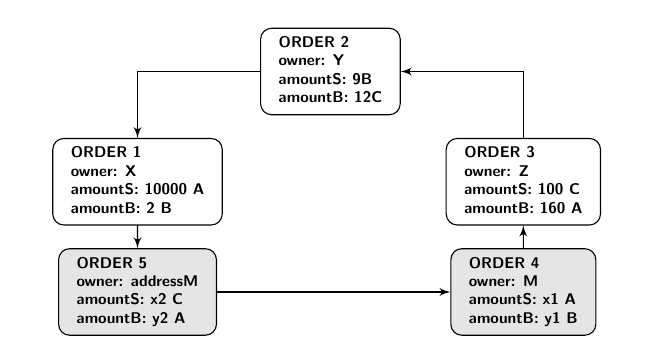
\begin{tikzpicture}[
    auto, 
    node distance=2cm,
    >=latex',
    font=\bfseries\footnotesize\sffamily,
    order/.style={
		scale=0.7,
		rectangle,
		rounded corners,
		draw=black, 
		text centered,
%		text width=5cm,
		minimum height=12mm,
		fill=white
	},
	label/.style={
		scale=0.7
	}
  ]
    % We start by placing the blocks

  \node [order] (order2) 
 {%
 \begin{tabular}{l}
  \textbf{ORDER 2}\\
  \textbf{owner: Y}\\
  \textbf{amountS: 9B}\\
  \textbf{amountB: 12C}
 \end{tabular}
 };
 
  \node [order, below of=order2, xshift=-3.5cm] (order1) 
 {%
 \begin{tabular}{l}
  \textbf{ORDER 1}\\
  \textbf{owner: X}\\
  \textbf{amountS: 10000 A}\\
  \textbf{amountB: 2 B}
 \end{tabular}
 };
 
 
  \node [order, below of=order2, xshift=3.5cm] (order3) 
 {%
 \begin{tabular}{l}
  \textbf{ORDER 3}\\
  \textbf{owner: Z}\\
  \textbf{amountS: 100 C}\\
  \textbf{amountB: 160 A}
 \end{tabular}
 };
 
   \node [order, below of=order3, fill=gray!20] (order4) 
 {%
 \begin{tabular}{l}
  \textbf{ORDER 4}\\
  \textbf{owner: M}\\
  \textbf{amountS: x1 A}\\
  \textbf{amountB: y1 B}
 \end{tabular}
 };
 
 
  \node [order, below of=order1, fill=gray!20] (order5) 
 {%
 \begin{tabular}{l}
  \textbf{ORDER 5}\\
  \textbf{owner: addressM}\\
  \textbf{amountS: x2 C}\\
  \textbf{amountB: y2 A}
 \end{tabular}
 };
 
 \draw [draw,->] (order1) -- node [label, xshift=-2cm] {} (order5);
 \draw [draw,->] (order2) -| node [label, xshift=-1.6cm] {} (order1);
 \draw [draw,->] (order3) |- node [label, xshift=1cm] {} (order2);
 \draw [draw,->] (order4) -- node [label, xshift=1.8cm] {} (order3);
 \draw [draw,->] (order5) -- node [label, yshift=0.2cm] {} (order4);
  
\end{tikzpicture}

\caption{An order-ring with sub-ring}
\label{fig:subring}
\end{figurehere}
\end{center}

This is zero-risk, zero-value add to the network, and is considered unfair conduct by the ring-miner. To prevent this, Loopring requires that a valid loop cannot contain any sub-rings. To check this, the LPSC ensures a token cannot be in a buy or sell position twice. In the above diagram, we can see that token \verb|A| is a sell token twice and a buy token twice, which would be disallowed. 


\subsubsection{Fill Rate Checking\label{sec:fill_rate_check}}


The exchange rate calculations in the order-ring are made by ring-miners for reasons stated above. It is the LPSC that must verify they're correct. First, it verifies that the buy rate the ring-miner can execute for each order is equal to or less than the original buy rate set by the user. This ensures the user gets at least the exchange rate they asked for or better on the transaction. Once the exchange rates are confirmed, the LPSC ensures that each order in the order-ring shares the same rate discount. For instance, if the discounted rate is $\gamma$, then the price for each order will be:

$r_{0\rightarrow 1} \cdot (1-\gamma)$, $r_{1\rightarrow 2} \cdot (1-\gamma)$, $r_{2 \rightarrow 0} \cdot (1-\gamma)$, and satisfy: 
\begin{equation}
r_{0\rightarrow 1} \cdot (1-\gamma)\cdot r_{1\rightarrow 2} \cdot (1-\gamma) \cdot r_{2 \rightarrow 0} \cdot (1-\gamma) = 1
\end{equation}
hence: 
\begin{equation}
\gamma = 1- \frac{1}{\sqrt[3]{r_{0\rightarrow 1} \cdot r_{1\rightarrow 2} \cdot r_{2\rightarrow 0}}}\text{.}
\end{equation}
If the transaction crosses $n$ orders, the \texttt{discount} is: 
\begin{equation}
\gamma = 1- \frac{1}{\sqrt[n]{\prod_{i=0}^{n-1} r^i}} \text{,}
\end{equation}

where $r^i$ is the order turnover rate of $i$-th order. Obviously, only when the discount rate is $\gamma \ge 0$, can these orders be filled; and the $i$-th order ($O^i$)'s actual exchange rate is $\hat{r^i} = r^i \cdot (1-\gamma)$, $\hat{r^i}\le r^i$.

Recall our prior example where Alice has 15 token \verb|A| and wants 4 token \verb|B| for them, Bob has 10 token \verb|B| and wants 30 token \verb|A| for them. If token \verb|A| is the reference, then Alice is buying token \verb|B| for $\frac{15}{4}$ = 3.75\verb|A|, while Bob is selling token \verb|B| for $\frac{30}{10}$ = 3.00\verb|A|. To calculate the discount: $\frac{150}{120}$ = 1.25 thus $\frac{1}{1.25}$ = 0.8 = $(1 −- \gamma)^2$. Thus the exchange rate that renders the trade equitable for both parties is $\sqrt{0.8}$ $\cdot$ 3.75 $\approx$ 3.3541 token \verb|A| per token \verb|B|.

Bob gives 4 token \verb|B| and receives 13.4164 token \verb|A|, more than the 12 he was expecting for those 4 tokens. Alice receives 4 token \verb|B| as intended but gives only 13.4164 token \verb|A| in exchange, less than the 15 she was willing to give for those 4 tokens.
Note, a portion of this margin will go towards paying fees to incentivize miners (and wallets). (See section \ref{sec:fee_model}).


\subsubsection{Fill Tracking \& Cancellation}

A user can partially or fully cancel an order by sending a special transaction to the LPSC, containing the details about the order and the amounts to cancel. The LPSC takes that into account, stores the amounts to cancel, and emits an \verb|OrderCancelled| event to the network. The LPSC keeps track of filled and cancelled amounts by storing their values using the order's hash as an identifier. This data is publicly accessible and \verb|OrderCancelled| / \verb|OrderFilled| events are emitted when it changes. Tracking these values is critical for the LPSC during the order-ring settlement step.

LPSC also supports cancelling all orders for any trading pair with the \verb|OrdersCancelled| event  and cancelling all orders for an address with the \verb|AllOrdersCancelled| event.


\subsubsection{Order Scaling\label{sec:order_scaling}}
Orders are scaled according to the history of filled and cancelled amounts and the current balance of the senders' accounts. The process finds the order with the smallest amount to be filled according to the above characteristics and uses it as a reference for scaling all transactions in the order-ring.


Finding the lowest value order can help to figure out the fill volume for each order. For instance, if the $i$-th order is the lowest value order, then the number of tokens sold from each order $\hat{s}$ and number of tokens purchased $\hat{b}$ from each order can be calculated as:

\[
\begin{split}
&\hat{s}^{i}=\overline{s}_i\text{, } \hat{b}^{i}=\hat{s}^{i}/ \hat{r}^i\text{, }\text{;}\\
&\hat{s}^{i\oplus 1}=\hat{b}^i\text{, } \hat{b}^{i\oplus 1}=\hat{s}^{i\oplus 1}/ \hat{r}^{i\oplus 1}\text{;}\\
&\hat{s}^{i\oplus 2}=\hat{b}^{i\oplus 1}\text{, } \hat{b}^{i\oplus 2}=\hat{s}^{i\oplus 2}/ \hat{r}^{i\oplus 2}\text{;}\\
& ...
%\text{.}
\end{split}
\]
where $\overline{s}_i$ is the balance left after orders are partially filled.

During implementation we can safely assume any order in the order-ring to have the lowest value, then iterate through the order-ring at most twice to calculate each order's fill volume. 

Example: If the smallest amount to be filled compared to the original order is 5\%, all the transactions in the order-ring are scaled down to 5\%. Once the transactions are completed, the order that was considered to have the smallest amount remaining to be filled should be completely filled.

\subsection{Ring Settlement\label{sec:settlement}}

If the order-ring fulfills all the previous checks, the order-ring can be closed, and transactions can be made. This means that all $n$ orders form a closed order-ring, connected as in figure 4:

\begin{center}
\begin{figurehere}
\centering
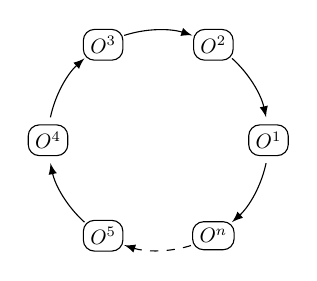
\begin{tikzpicture}[
circle/.style={
		scale=0.75,
		rounded corners,
		draw=black, 
		text centered,
		}
]

\def \n {6}
\def \m {4}
\def \radius {1.4cm}
\def \margin {12} % margin in angles, depends on the radius

\foreach \s in {1,...,\m}
{
  \node[draw, circle] at ({360/\n * (\s - 1)}:\radius) {$O^\s$};
  \draw[<-, >=latex] ({360/\n * (\s - 1)+\margin}:\radius) 
    arc ({360/\n * (\s - 1)+\margin}:{360/\n * (\s)-\margin}:\radius);
}

\node[draw, circle] at ({360/\n * 4}:\radius) {$O^5$};
  \draw[<-, dashed, >=latex] ({360/\n * 4+\margin}:\radius) 
    arc ({360/\n * 4+\margin}:{360/\n * (5)-\margin}:\radius);
    
\node[draw, circle] at ({360/\n * 5}:\radius) {$O^n$};
  \draw[<-, >=latex] ({360/\n * 5+\margin}:\radius) 
    arc ({360/\n * 5+\margin}:{360/\n * (6)-\margin}:\radius);


\end{tikzpicture}
\caption{Ring Settlement}
\label{fig:settlement}
\end{figurehere}
\end{center}

To make the transactions, the LPSC uses the \verb|TokenTransferDelegate| smart contract. The introduction of such a delegate makes upgrading the protocol smart contract easier as all orders only need to authorize this delegate instead of different versions of the protocol.

For each order in the order-ring, a payment of \verb|tokenS| is made to the next or the previous order depending on the implementation. Then the ring-miner's fee is paid depending on the fee model chosen by the ring-miner. Finally, once all the transactions are made, a \verb|RingMined| event is emitted.

\subsubsection{Emitted Events\label{sec:events}}

The protocol emits events that allow relays, order browsers, and other actors to receive order book updates as efficiently as possible. The emitted events are:

\begin{itemize}
	\item \textbf{OrderCancelled}: A specific order has been cancelled.
	\item \textbf{OrdersCancelled}: All orders of a trading pair from an owning address have been cancelled.
	\item \textbf{AllOrdersCancelled}: All orders of all trading pairs from an owning address have been cancelled.
	\item \textbf{RingMined}: An order-ring has been settled successfully. This event contains data related to each inner-ring token transfer.
\end{itemize}


\section{LRx Token\label{sec:token}}
LRx is our generalized token notation. LRC is the Loopring token on Ethereum, LRQ on Qtum, and LRN on NEO, etc. Other LRx types will be introduced in the future as Loopring is deployed on other public blockchains.

\subsection{Fee Model\label{sec:fee_model}} 
When a user creates an order, they specify an amount of LRx to be paid to the ring-miner as a fee, in conjunction with a percentage of the margin (\verb|marginSplitPercentage|) made on the order that the ring-miner can claim. This is called the margin split. The decision of which one to choose (fee or margin split) is left to the ring-miner.

A representation of the margin split:

\begin{center}
\begin{figurehere}
\centering
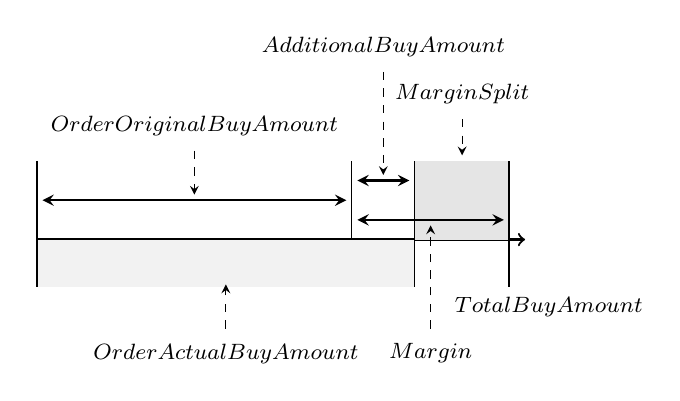
\begin{tikzpicture}[
scale=1,
font=\bfseries\footnotesize\sffamily,
classical/.style={thick,<->,shorten >=2pt,shorten <=2pt,>=stealth},
oneway/.style={->,dashed,shorten >=2pt,shorten <=2pt,>=stealth}
]
    % Draw axes
    \draw [->,thick] (0,1) node (yaxis) [above] {$$}
        |- (6.2,0) node (xaxis) [right] {$$};
        
    \draw
  	(4,0) coordinate (A)
  	(4,1) coordinate (A2)
  	(4.8,-0.6) coordinate (B)
  	(4.8,1) coordinate (B2)
  	(6,-0.6) coordinate (C)
  	(6,1) coordinate (C2);
  	
  	\fill [draw=none, fill=gray!20] 
    (4.8, 0) rectangle (6, 1);
    
  	\fill [draw=none, fill=gray!10] 
    (0, -0.6) rectangle (4.8, 0);

	\draw[thick] (0, -0.6) -- (0, 0.6) node[below]{$$};
  	\draw[thick, thin] (A) -- (A2) node[below]{$$};
  	\draw[thick, thin] (B) -- (B2) node[below]{$$};
  	\draw[thick] (C) node[below, xshift=0.5cm]{$Total Buy Amount$} -- (C2) ;
  	
  	\draw[classical] (0, 0.5) -> (4, 0.5) node[below]{$$};
  	\draw[classical] (4, 0.75) -> (4.8, 0.75) node[below]{$$};
%  	\draw[classical] (4.8, 0.5) -> (6, 0.5) node[below]{$$};
  	\draw[classical] (4, 0.25) -> (6, 0.25) node[below]{$$};

  	
  	\draw[oneway] (2, 1.2) node[above]{$Order Original Buy Amount$} -- (2, 0.5);
  	\draw[oneway] (4.4, 2.2) node[above]{$Additional Buy Amount$} -- (4.4, 0.75);
  	\draw[oneway] (5.4, 1.6) node[above]{$Margin Split$} -- (5.4, 1);
  	\draw[oneway] (5, -1.2) node[below]{$Margin$} -- (5, 0.25);
  	\draw[oneway] (2.4, -1.2) node[below]{$Order Actual Buy Amount$} -- (2.4, -0.5);



\end{tikzpicture}
\caption{A 60\% Margin Split}
\label{fig:marginsplit}
\end{figurehere}
\end{center}

If the margin on the order-ring is too small, a ring-miner will choose the LRx fee. If, on the contrary, the margin is substantial enough for the resulting margin split to be worth much more than the LRx fee, a ring-miner will choose the margin split. There is another proviso, however: when the ring-miner chooses the margin split, they must pay the user (order creator) a fee, which is equal to the LRx the user would have paid to the ring-miner as a fee. This increases the threshold of where the ring-miner will choose the margin split to twice the LRx fee of the order, increasing the propensity of the LRx fee choice. This allows ring-miners to receive a constant income on low margin order-rings for the tradeoff of receiving less income on higher margin order-rings. Our fee model is based on the expectation that as the market grows and matures, there will be fewer high margin order-rings, thus necessitating fixed LRx fees as incentive.


We end up with the following graph:

\begin{center}
\begin{figurehere}
\centering
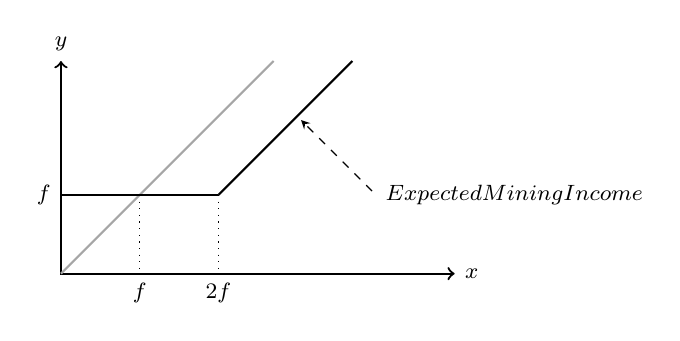
\begin{tikzpicture}[
font=\bfseries\footnotesize\sffamily,
oneway/.style={->,dashed,shorten >=2pt,shorten <=2pt,>=stealth},
scale=1]
    % Draw axes
    \draw [<->,thick] (0,2.7) node (yaxis) [above] {$y$}
        |- (5,0) node (xaxis) [right] {$x$};
        
    \draw
  	(1,1) coordinate (A)
  	(2,1) coordinate (B);
  	
  	
  	\draw[thick] (B) -- (3.7,2.7);
  	\draw[dotted] (B) -- (2,0) node[below] {$2f$};
  	\draw[dotted] (A) -- (1,0) node[below] {$f$};
  	\draw[thick,color=gray!70] (0,0) -- (2.7,2.7);
  	\draw[thick] (0,1) node[left] {$f$}--(B) node[     ]{$$};
 	\draw[oneway] (4,1) node[right]{$Expected Mining Income$} -- (3, 2);


\end{tikzpicture}
\caption{Loopring's Fee Model}
\label{fig:feemodel}
\end{figurehere}
\end{center}


where $f$ is the LRx fee, $x$ is the margin split, $y$ is the mining income. $y=max(f, x-f)$ as indicated by the solid line; if the LRx fee for the order is $0$, the equation is $y=max(0, x - 0)$ that simplifies to $y=x$ as indicated by the gray line.


The consequences are:  
\begin{enumerate}
	\item If the margin split is 0, ring-miners will choose the flat LRx fee and are still incentivized. 
	\item If the LRx fee is 0, the gray line results and the income is based on a general linear model.
	\item When the margin split income is greater than 2x(LRx fee), ring-miners choose the margin split and pay LRx to the user.
\end{enumerate}

It should be noted that if the LRx fee is non-zero, no matter which option the ring-miner chooses, there will always be a transfer of LRx between the ring-miner and the order's sender. Either the ring-miner earns the LRx fee, or pays the LRx fee back to the sender to take the margin split.

Ring-miners will share a certain percentage of fees with wallets. When a user places an order through a wallet and gets filled, the wallet is rewarded with a portion of the fees or margin split. Although this is modular, and unique business models or implementations are possible, our inclination is for wallets to receive approximately 20\%-25\% of earned fees. Wallets represent a primary target for Loopring protocol integration as they have the user base, but little or no source of income.

\subsection{Decentralized Governance}
At its root, the Loopring protocol is a social protocol in the sense that it relies on coordination amongst members to operate effectively towards a goal. This is not dissimilar to cryptoeconomic protocols at large, and indeed, its usefulness is largely protected by the same mechanisms of coordination problems \cite{vitalikgovernance}, grim trigger equilibrium, and bounded rationality. To this end, LRx tokens are not only used to pay fees, but also to align the financial incentives of the various network participants. Such alignment is necessary for broad adoption of any protocol, but is particularly acute for exchange protocols, given that success rests largely on improving liquidity in a robust decentralized ecosystem.

LRx tokens will be used to effectuate protocol updates through decentralized governance. Smart contract updates will, in part, be governed by token holders to ensure continuity and safety, and to attenuate the risks of siphoned liquidity through incompatibility. Given that smart contracts cannot be altered once deployed, there is a risk that dApps or end users continue to interact with deprecated versions and preclude themselves from updated contracts. Upgradeability is crucial to the protocol's success as it must adapt to market demands and the underlying blockchains. Decentralized governance by LRx stakeholders will allow for protocol smart contract updates without disrupting dApps or end users, or relying too heavily on smart contract abstraction. LRx tokens have a fixed supply, and in the case of LRC, certain percentages are frozen from the Loopring Foundation, and allocated to community-purposed funds \cite{LRCtokendoc}.

However, LRx token owners are not the only stakeholders to consider in steering the protocol's direction: relays/ring-miners, wallets, developers, and others are an integral part of the ecosystem and their voice must be heard. In fact, given that these agents need not hold any LRx to perform their respective roles (since traditional makers/takers and market-makers are nonexistent, initial token reserves are not mandatory) we must allow alternative methods for their interests to be respected. Furthermore, "simple" token-based voting, both on-chain and off, is an imperfect salve for disagreement, as low voter turnout and token ownership concentration pose risks. Thus, the goal is to implement a governance model that is built in layers, and rests on a shared knowledge that some set of decision-making processes is the norm. This can be facilitated by coordination institutions that offer signals from a diverse set of participants, and, perhaps, from pre-established protocol focal points. As this comes to fruition, the Loopring Foundation will inevitably evolve from protocol developers into protocol stewards.

\section{Fraud and Attack Protections}

\subsection{Front-running Prevention\label{sec:dual_authoring}}

In decentralized exchanges, front-running is when someone tries to copy another node's trade solution, and have it mined before the original transaction that is in the pending transaction pool (mempool). This can be achieved by specifying a higher transaction fee (gas price). The major scheme of front-running in Loopring (and any protocol for order-matching) are order-filch: when a front-runner steals one or more orders from a pending order-ring settlement transaction; and, specific to Loopring: when a front-runner steals the entire order-ring from a pending transaction.


When a submitRing transaction is not confirmed and is still in the pending transaction pool, anyone can easily spot such a transaction and replace \verb|minerAddress| with their own address (the \verb|filcherAddress|), then they can re-sign the payload with \verb|filcherAddress| to replace the order-ring's signature. The filcher can set a higher gas price and submit a new transaction hoping block-miners will pick his new transaction into the next block instead of the original submitRing transaction.

Previous solutions to this problem had important downsides: requiring more transactions and thus costing ring-miners more gas; and taking at least twice the blocks to settle an order-ring.  Our new solution, Dual Authoring\cite{dualauthor}, involves the mechanism of setting up two levels of authorization for orders - one for settlement, and one for ring-mining.

Dual Authoring process:

\begin{enumerate}

	\item For each order, the wallet software will generate a random public-key/private-key pair, and put the key pair into the order's JSON snippet. (An alternative is to use the address derived from the public-key instead of the public-key itself to reduce byte size. We use \verb|authAddr| to represent such an address, and \verb|authKey| to represent \verb|authAddr|'s matching private-key).

	\item Compute the order's hash with all fields in the order except \verb|r|, \verb|v|, \verb|s|, and \verb|authKey|), and sign the hash using the \verb|owner|'s private-key (not \verb|authKey|).

	\item The wallet will send the order together with the \verb|authKey| to  relays for ring-mining. Ring-miners will verify that \verb|authKey| and \verb|authAddr| are correctly paired and the order's signature is valid with respect to \verb|owner| address.

	\item When an order-ring is identified, the ring-miner will use each order's \verb|authKey| to sign the ring's hash, \verb|minerAddress|, and all the mining parameters. If an order-ring contains $n$ orders, there will be $n$ signatures by the $n$ \verb|authKey|s. We call these signatures the \verb|authSignature|s. The ring-miner may also need to sign the ring's hash together with all mining parameters using \verb|minerAddress|'s private-key.

	\item The ring-miner calls the submitRing function with all the parameters, as well as all the extra \verb|authSignature|s. Notice that \verb|authKey|s are NOT part of the on-chain transaction and thus remain unknown to parties other than the ring-miner itself.


	\item The Loopring Protocol will now verify each \verb|authSignature| against the corresponding \verb|authAddr| of each order, and reject the order-ring if any \verb|authSignature| is missing or invalid.
 
\end{enumerate}

The result is that now:

\begin{itemize}

	\item  The order's signature (by the private-key of the \verb|owner| address) guarantees the order cannot be modified, including the \verb|authAddr|.
	\item  The ring-miner's signature (by the private-key of the \verb|minerAddress|), if supplied, guarantees nobody can use his identity to mine an order-ring.
	\item  The \verb|authSignature|s guarantees the entire order-ring cannot be modified, including \verb|minerAddress|, and no orders can be stolen.

\end{itemize}

Dual Authoring prevents ring-filch and order-filch while still ensuring the settlement of order-rings can be done in one single transaction. In addition, Dual Authoring opens doors for relays to share orders in two ways: non-matchable sharing and matchable sharing. By default, Loopring operates an OTC model and only supports limit-price orders, meaning that orders' timestamps are ignored. This implies that front-running a trade has no impact on the actual price of that trade, but does impact whether it gets executed or not.

\section{Other Attacks}

\subsection{Sybil or DOS Attack}
Malicious users -- acting as themselves or forged identities -- could send a large amount of small orders to attack Loopring nodes. However, since we allow nodes to reject orders based on their own criteria -- which they may hide or reveal -- most of these orders will be rejected for not yielding satisfying profit when matched.  By empowering relays to dictate how they manage orders, we do not see a massive tiny order attack as a threat.

\subsection{Insufficient Balance}
Malicious users could sign and spread orders whose order value is non-zero but whose address actually has zero balance. Nodes could monitor and notice that some orders actual balance is zero, update these order states accordingly and then discard them.
Nodes must spend time to update the status of an order, but can also choose to minimize the effort by, for example, blacklisting addresses and dropping related orders.

\section{Summary}

The Loopring protocol sets out to be a foundational layer for decentralized exchange. In so doing, it has profound repurcussions in how people exchange assets and value. Money, as an intermediate commodity, facilitates or replaces barter exchange and solves the double coincidence of wants problem \cite{unenumerated2006}, whereby two counterparties must desire each other's distinct good or service. Similarly, Loopring protocol aims to dispense of our dependencies on coincidence of wants in trading pairs, by using ring matching to more easily consummate trades. This is meaningful for how society and markets exchange tokens, traditional assets, and beyond. Indeed, just as decentralized cryptocurrencies pose threat to a nation's control over money, a combinatorial protocol that can match traders (consumers/producers) at scale, is a theoretical threat to the concept of money itself.

Protocol benefits include:

\begin{itemize}
	\item Off-chain order management and on-chain settlement means no sacrifice in performance for security.
	\item Greater liquidity due to ring-mining and order sharing.
	\item Dual Authoring solves the pernicious problem of front running faced by all DEXs and their users today.
	\item Free, public smart contracts enable any dApp to build or interact with the protocol.
	\item Standardization among operators allows for network effects and an improved end user experience.
	\item Network maintained with flexibility in running order books and communicating.
	\item Reduced barriers to entry means lower costs for nodes joining the network and end users.
	\item Anonymous trading directly from user wallets.
\end{itemize}

\section{Acknowledgements}
We would like to express our gratitude to our mentors, advisers and to the many people in the community that have been so welcoming and generous with their knowledge. In particular, we would like to thank Shuo Bai (from ChinaLedger); Professor Haibin Kan; Alex Cheng, Hongfei Da; Yin Cao; Xiaochuan Wu; Zhen Wang, Wei Yu, Nian Duan, Jun Xiao, Jiang Qian, Jiangxu Xiang, Yipeng Guo, Dahai Li, Kelvin Long, Huaxia Xia, Jun Ma, and Encephalo Path for reviewing and providing feedback on this project. 


\bibliography{whitepaper}
\bibliographystyle{unsrt}


\end{multicols}


\begin{appendices}

\section{Loopring Implemented on EVM\label{app:protocol_ethereum}}

\begin{center}
\begin{figurehere}
\centering
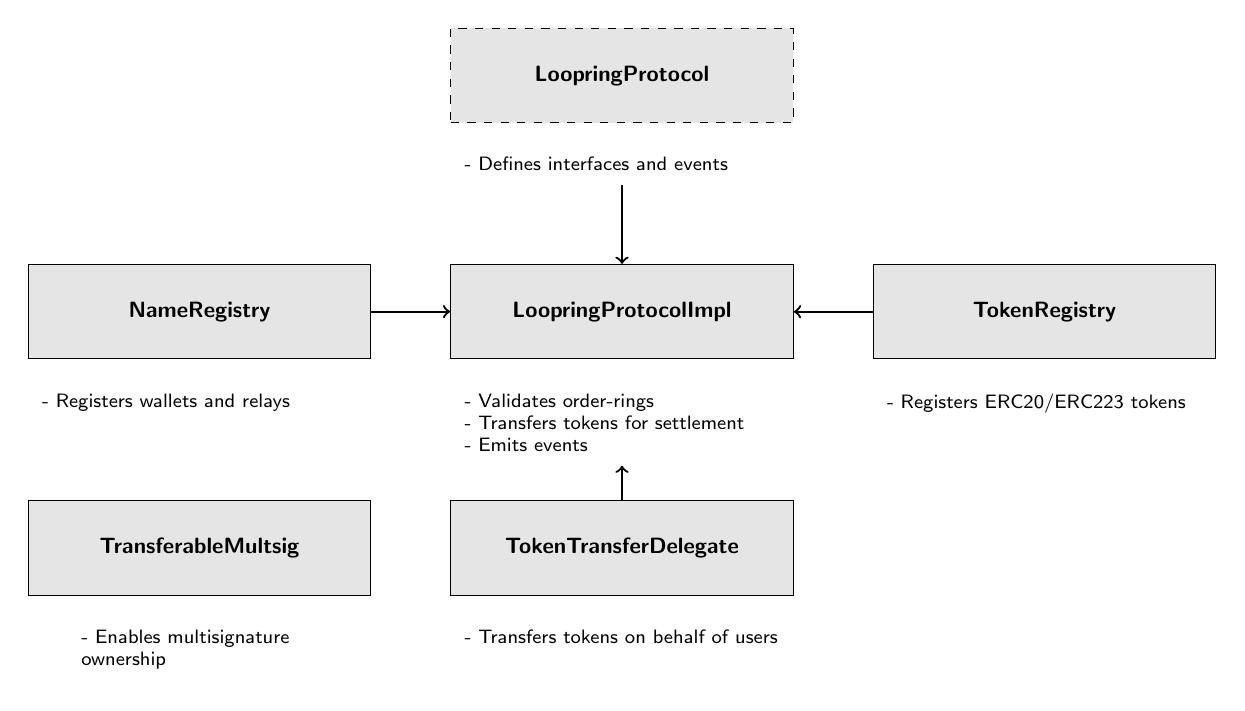
\begin{tikzpicture}
[node distance = 1cm, auto,font=\footnotesize,
% STYLES
every node/.style={node distance=3cm},
% The comment style is used to describe the characteristics of each force
comment/.style={rectangle, inner sep= 5pt, text width=4cm, node distance=0.25cm, font=\scriptsize\sffamily},
% The force style is used to draw the forces' name
force/.style={rectangle, draw, fill=black!10, inner sep=5pt, text width=4cm, text badly centered, minimum height=1.2cm, font=\bfseries\footnotesize\sffamily}] 

% Draw forces
\node [force] (impl) {LoopringProtocolImpl};
\node [force, dashed, above of=impl] (protocol_interface) {LoopringProtocol};
\node [force, left=1cm of impl] (nameregistry) {NameRegistry};
\node [force, right=1cm of impl] (tokenregistry) {TokenRegistry};
\node [force, below of=impl] (delegate) {TokenTransferDelegate};
\node [force, left=1cm of delegate] (multisig) {TransferableMultsig};

%%%%%%%%%%%%%%%
% Change data from here

% impl
\node [comment, below=0.25 of impl] (comment-impl) {- Validates order-rings\\
- Transfers tokens for settlement\\
- Emits events};

% nameregistry
\node [comment, below=0.25cm of nameregistry]{- Registers wallets and relays};

% protocol_interface
\node [comment, below=0.25 of protocol_interface](comment-interface) {- Defines interfaces and events};

% tokenregistry
\node [comment, below=0.25 of tokenregistry] {- Registers ERC20/ERC223 tokens};

% delegate
\node [comment, below=0.25 of delegate] {- Transfers tokens on behalf of users};

% PUBLIC POLICIES
\node [comment, text width=3cm, below=0.25 of multisig] {- Enables multisignature ownership};

%%%%%%%%%%%%%%%%

% Draw the links between forces
\path[->,thick] 
(comment-interface) edge (impl)
(nameregistry) edge (impl)
(tokenregistry) edge (impl)
(delegate) edge (comment-impl);

\end{tikzpicture} 
\caption{Smart Contracts}
\label{fig:smartcontracts}
\end{figurehere}
\end{center}

\section{Deployment}


\subsection{Ethereum}
The following smart contracts have been deployed on Ethereum mainnet:
\begin{itemize}
\item LRC: \verb|0xEF68e7C694F40c8202821eDF525dE3782458639f|
\item TokenRegistry: \verb|0xa21c1f2AE7f721aE77b1204A4f0811c642638da9|
\item TokenTransferDelegate: \verb|0x7b126ab811f278f288bf1d62d47334351dA20d1d|
\item NameRegistry: \verb|0xd181c1808e3f010F0F0aABc6Fe1bcE2025DB7Bb7|
\item LoopringProtocolImpl: \verb|0x0B48b747436f10c846696e889e66425e05CD740f|
\end{itemize}

\subsection{Qtum}
The following smart contracts have been deployed on Qtum mainnet:
\begin{itemize}
\item LRQ: \verb| 2eb2a66afd4e465fb06d8b71f30fb1b93e18788d |
\item TokenRegistry: \verb| c89ea34360258917daf3655f8bec5550923509b3 |
\item TokenTransferDelegate: \verb| 60b3fa7f461664e4dafb621a36ac2722cc680f10 |
\item NameRegistry: \verb| e26a27d92181069b25bc7283e03722f6ce7678bb |
\item LoopringProtocolImpl: \verb| 5180bb56b696d16635abd8dc235e0ee432abf25d |
\end{itemize}

\end{appendices}
\end{document}
